% !TeX spellcheck = en_GB
\section{Skew-T log-P diagram from Stavanger}%\hfill} 
\label{app:sounding}
The Skew-T log-P diagram shows the observed vertical temperature and dew-point temperature at Stavanger. The data are taken from \cite{wyoming_atmospheric_2018} and processed in Python.

Isobars are grey lines, every \SI{50}{\hPa}, dry adiabats are blue (labelled in \SI{}{\celsius}), isotherms are red [\SI{}{\celsius}], water vapour mixing ratios are green, dashed in [\SI{}{\gram\per\kilogram}], and moist adiabats are dashed, purple lines (labelled in [\SI{}{\celsius}]).

\begin{landscape}
	\begin{figure}\ContinuedFloat
		\centering
		% 20/12
		\begin{subfigure}[b]{0.66\textheight}
			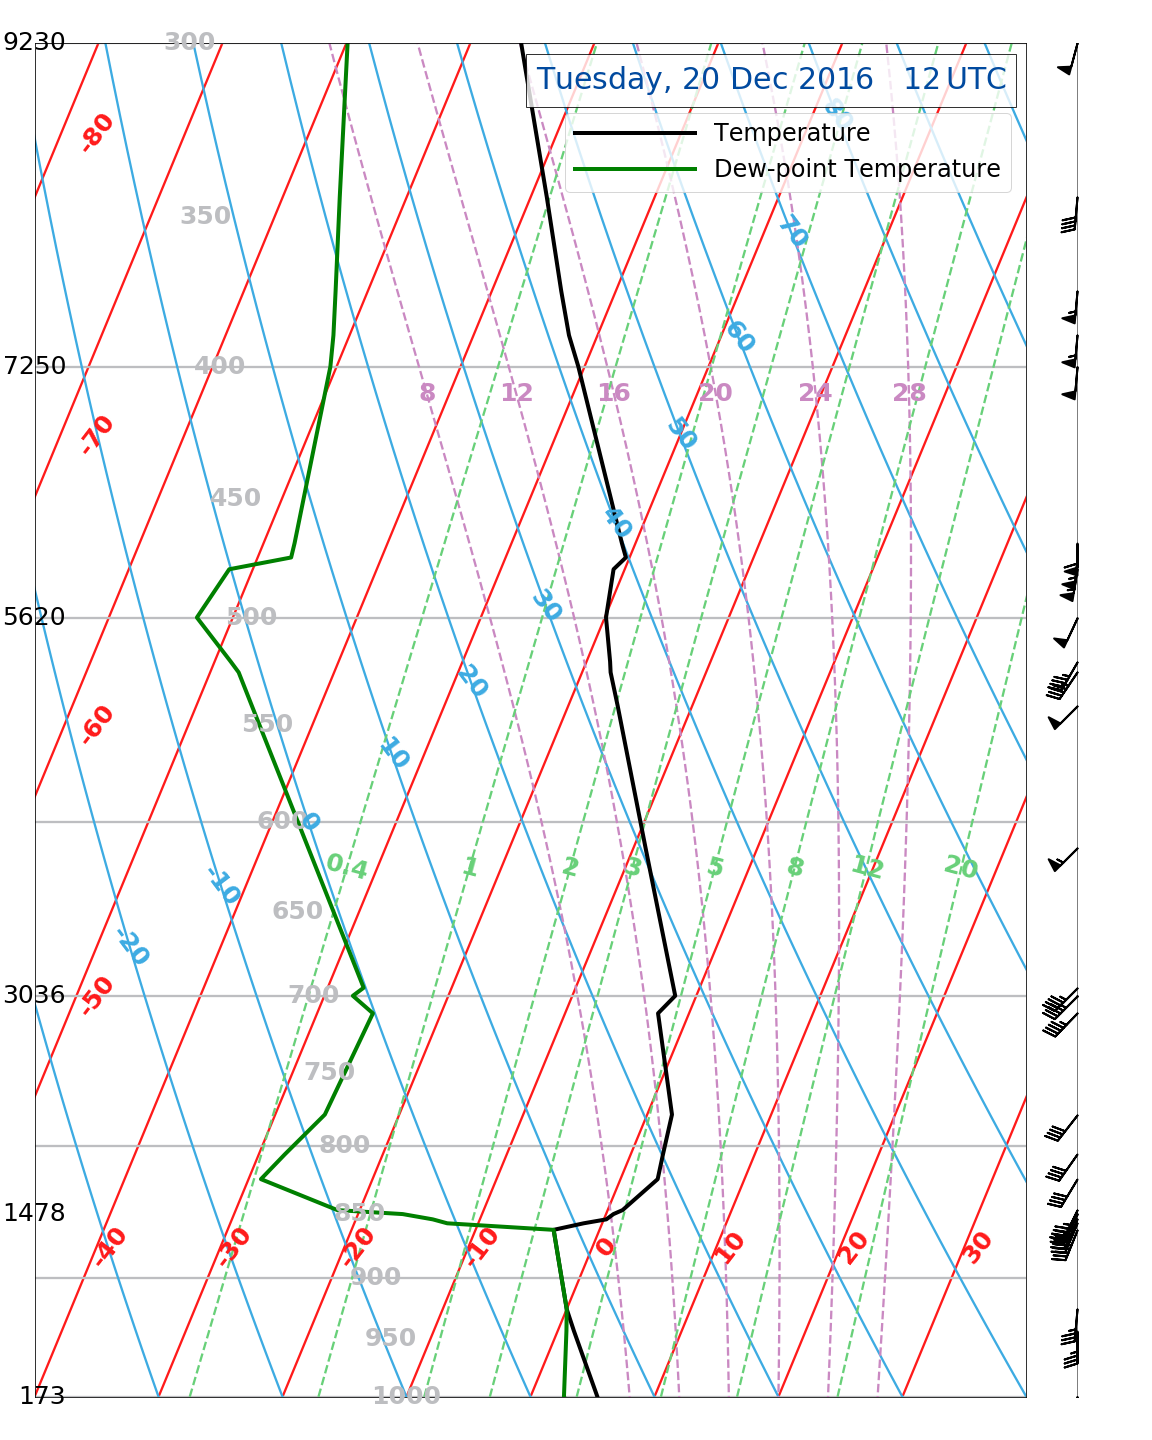
\includegraphics[trim={0cm 0.2cm 2.5cm .5cm},clip,width=\textwidth]{./fig_Sounding/20161220_12Z}
			\caption{}\label{fig:Soun20}
		\end{subfigure}
		\quad
		% 21/12
		\begin{subfigure}[b]{0.66\textheight}
			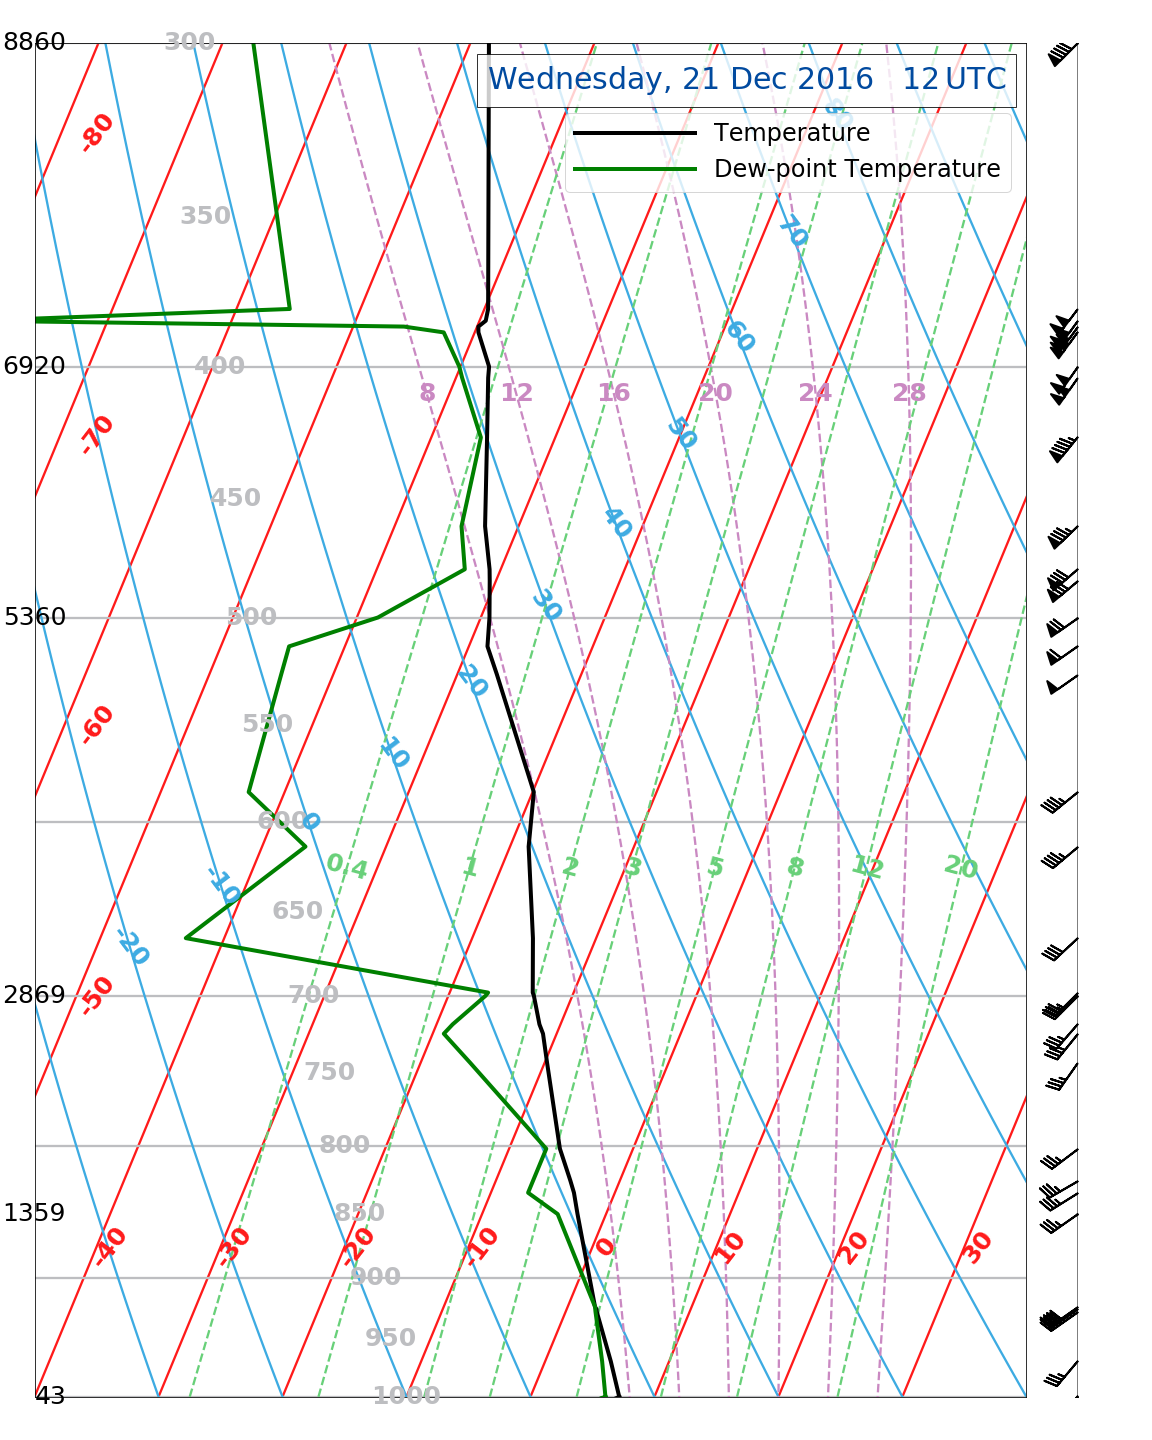
\includegraphics[trim={0cm 0.2cm 2.5cm .5cm},clip,width=\textwidth]{./fig_Sounding/20161221_12Z}
			\caption{}\label{fig:Soun21}
		\end{subfigure}
	\end{figure}
	
	%%%%%%%% 2nd page
	\begin{figure}\ContinuedFloat
		\centering
		% 22/12
		\begin{subfigure}[b]{0.66\textheight}
			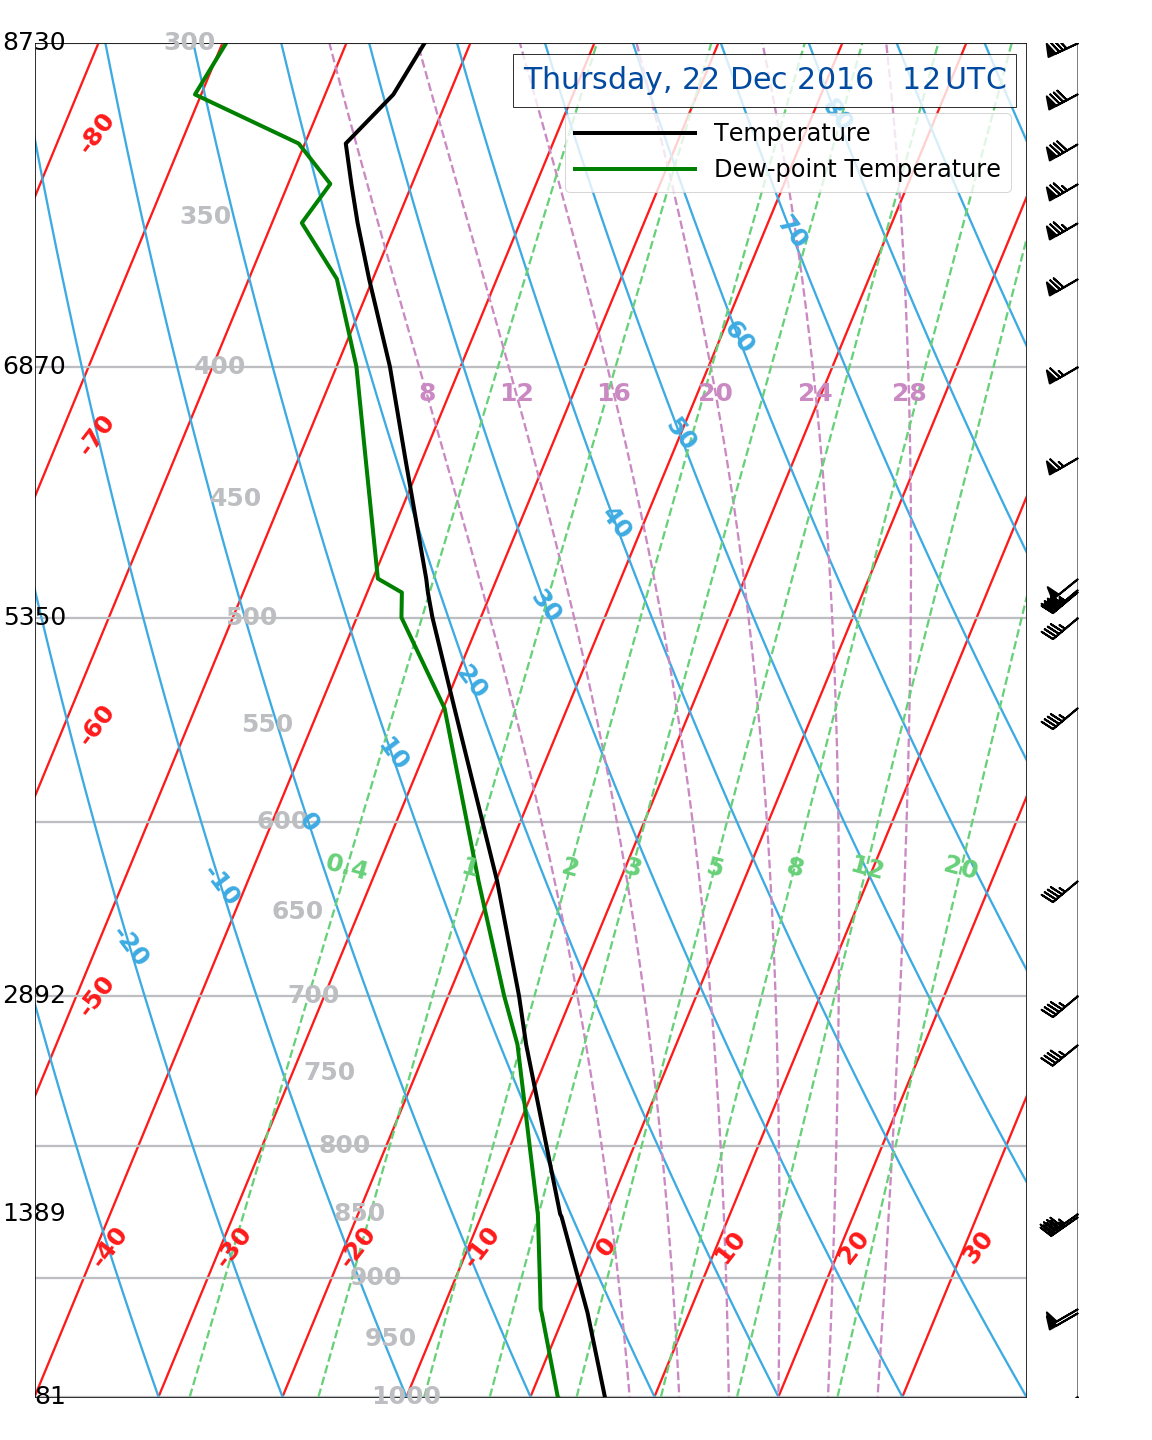
\includegraphics[trim={0cm 0.2cm 2.5cm .5cm},clip,
			width=\textwidth]{./fig_Sounding/20161222_12Z}
			\caption{}\label{fig:Soun22}
		\end{subfigure}
		\quad
		% 23/00
		\begin{subfigure}[b]{0.66\textheight}
			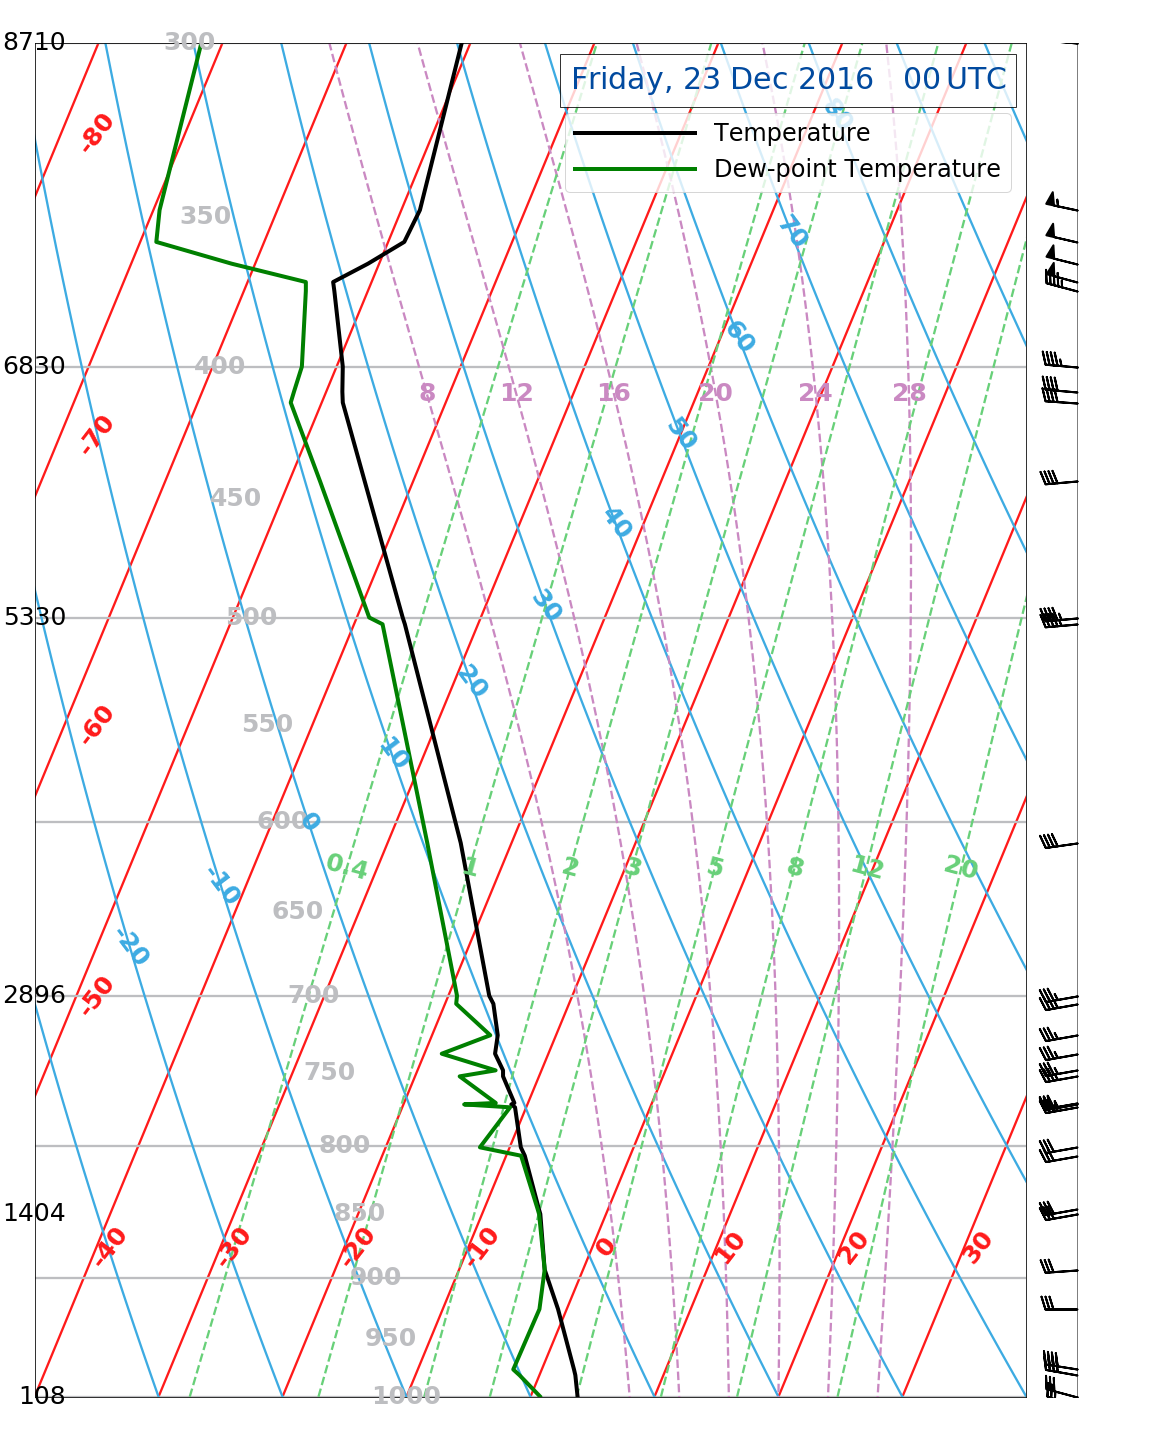
\includegraphics[trim={0cm 0.2cm 2.5cm .5cm},clip,
			width=\textwidth]{./fig_Sounding/20161223_00Z}
			\caption{}\label{fig:Soun23}
		\end{subfigure}
	\end{figure}
	
	%%%%%%%% 3rd page
	\begin{figure}\ContinuedFloat
		\centering
		% 25/12
		\begin{subfigure}[b]{0.66\textheight}
			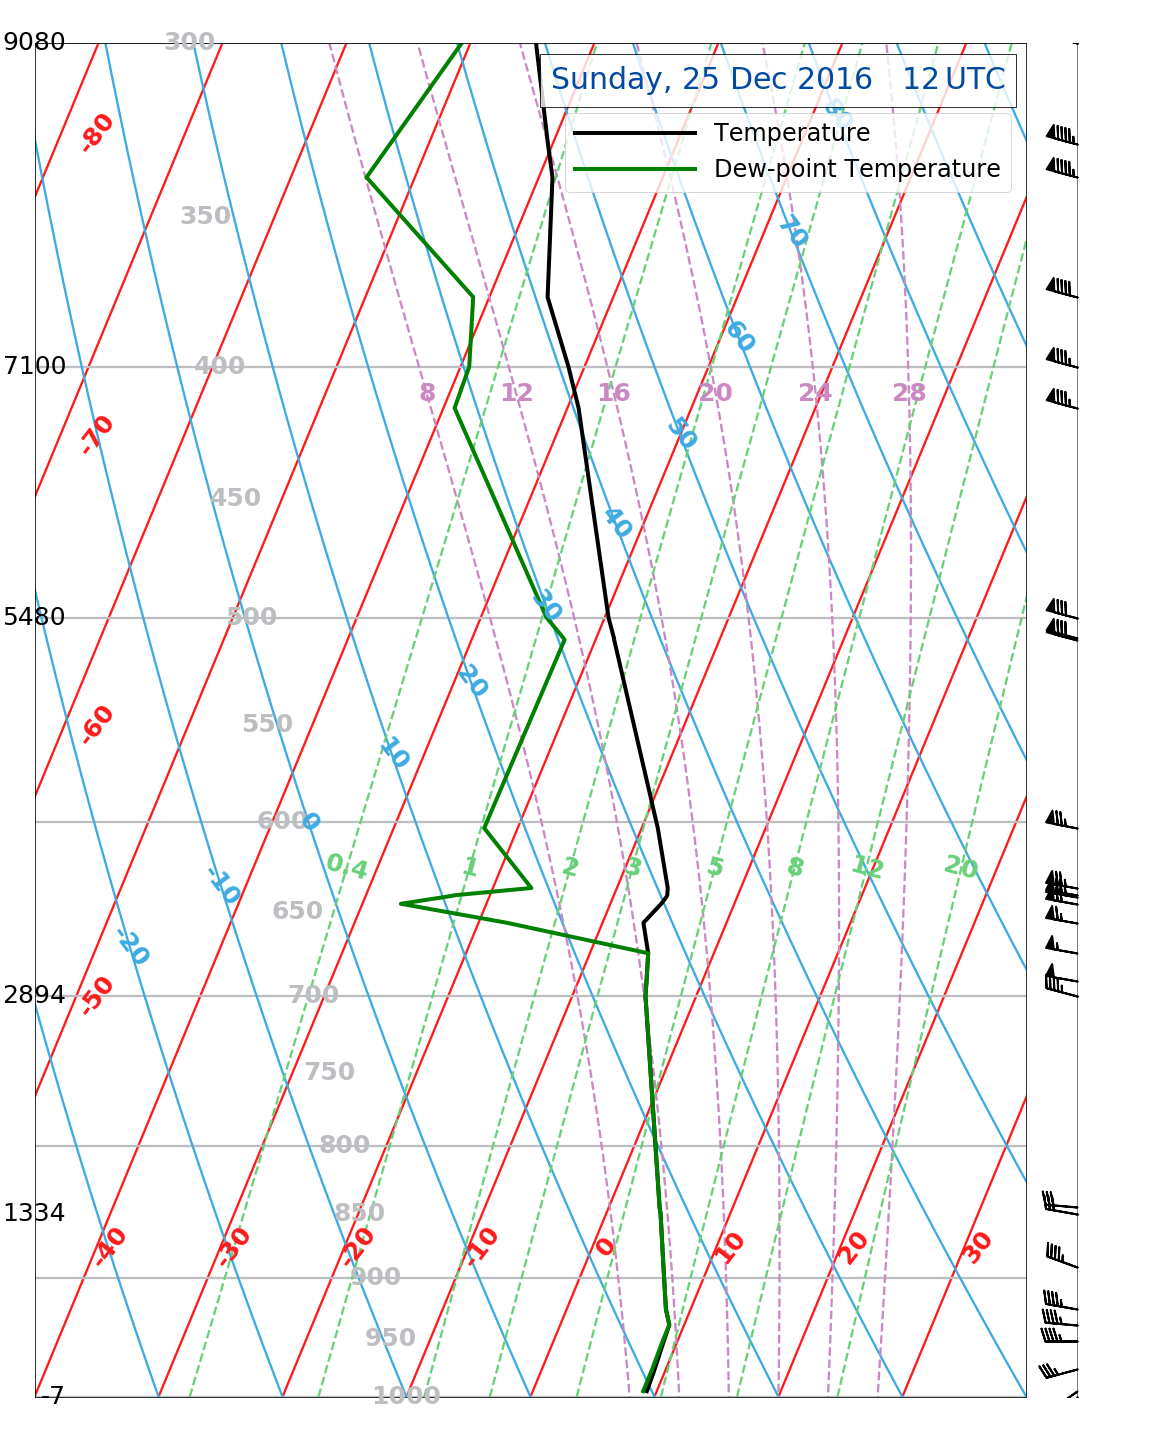
\includegraphics[trim={0cm 0.2cm 2.5cm .5cm},clip,
			width=\textwidth]{./fig_Sounding/20161225_12Z}
			\caption{}\label{fig:Soun25}
		\end{subfigure}
		\quad
		% 26/12
		\begin{subfigure}[b]{0.66\textheight}
			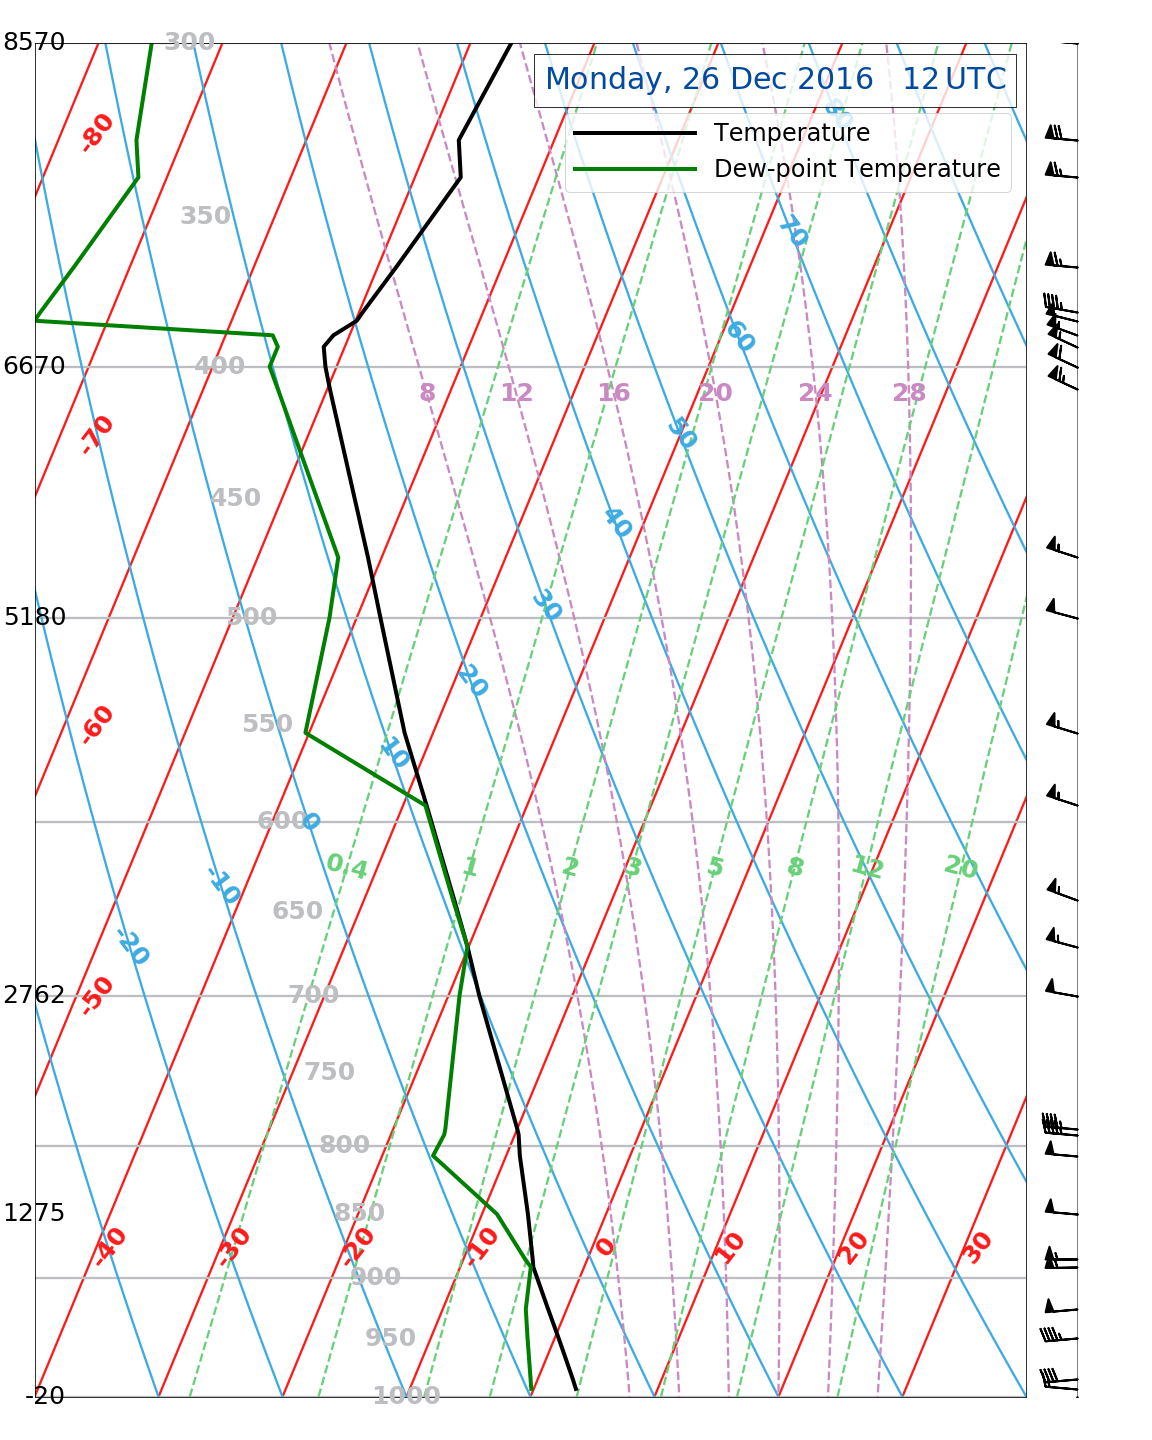
\includegraphics[trim={0cm 0.2cm 2.5cm .5cm},clip,
			width=\textwidth]{./fig_Sounding/20161226_12Z}
			\caption{}\label{fig:Soun26}
		\end{subfigure}
		
		\caption{Vertical profiles of atmospheric temperature (black) and dew-point temperature (green) during \SIrange{20}{26}{\dec}. Vertical Profiles from \SI{24}{\dec} are missing at the webpage \url{http://weather.uwyo.edu/upperair/sounding.html}}\label{fig:sounding}
	\end{figure}
\end{landscape}